\section{修正Newton法}
\label{sec:newton-modified}

上一节假定Hessian正定。这就需要回答：Hessian不定或接近奇异时，方向本身已经不可用，怎样改造曲率矩阵，既得到可靠的下降方向，又不破坏解附近的快速收敛？

\paragraph{缩短步长为什么不够}
在目标~\eqref{eq:newton-running-objective}的点$\bm{x}=(-\tfrac12,\tfrac34)$处，$u=\tfrac12$，由式~\eqref{eq:newton-running-derivatives}，
\[
 \bm{g}=\begin{bmatrix}-\tfrac12\\1\end{bmatrix},\qquad
 \bm{H}=\begin{bmatrix}1&2\\2&2\end{bmatrix}.
\]
$\bm{H}$的行列式是$-2$，特征值约为$3.56$和$-0.56$，不定。由式~\eqref{eq:newton-running-direction}，Newton方向是$\bm{d}=(-1.5,1)$，方向导数为
\[
 \bm{g}^\top\bm{d}=0.75+1=1.75>0.
\]
这是上坡方向，无论步长取多小，目标都上升。图~\ref{fig:newton-directions}中红色箭头正是这个方向，它指向离解更远的地方。

Hessian接近奇异时情形相反：方向是下坡的，但$\lVert\bm{d}\rVert_2$大得离谱。上一节$(-1,\tfrac65)$处的方向长度超过$22$，回溯要试探五次才找到可接受的步长。

问题出在模型的形状。负曲率方向上碗是倒扣的，几乎平坦的方向上碗底远在天边。于是不改步长，改曲率矩阵。

\paragraph{用正定矩阵代替Hessian}
\term{修正Newton法}（modified Newton method）用一个正定矩阵$\bm{B}^{(t)}$代替$\bm{H}^{(t)}$，解
\begin{equation}
 \bm{B}^{(t)}\bm{d}^{(t)}=-\bm{g}^{(t)},\qquad \bm{B}^{(t)}=\bm{H}^{(t)}+\bm{E}^{(t)}\succ\bm{0}.
 \label{eq:newton-modified-equation}
\end{equation}
其中$\bm{E}^{(t)}$是修正量。方向导数是
\[
 (\bm{g}^{(t)})^\top\bm{d}^{(t)}=-(\bm{g}^{(t)})^\top(\bm{B}^{(t)})^{-1}\bm{g}^{(t)}.
\]
$\bm{B}^{(t)}$正定，所以只要$\bm{g}^{(t)}\neq\bm{0}$，方向就是下降方向，上一节的回溯可以照用。

修正量的选择要在两种需求之间平衡。一方面希望$\bm{E}^{(t)}$足够大，让$\bm{B}^{(t)}$的条件数不太差。另一方面希望$\bm{E}^{(t)}$尽量小，因为它越大，模型离真实的曲率越远。Hessian本来就足够正定时，应当令$\bm{E}^{(t)}=\bm{0}$。下面三种常见做法，差别在于用什么代价换来多少修正。

\paragraph{对角平移}
最简单的修正是取$\bm{E}^{(t)}=\delta^{(t)}\bm{I}$：
\begin{equation}
 \bm{B}^{(t)}=\bm{H}^{(t)}+\delta^{(t)}\bm{I},\qquad \delta^{(t)}>\max\bigl\{0,-\lambda_{\min}(\bm{H}^{(t)})\bigr\}.
 \label{eq:newton-shift}
\end{equation}
所有特征值都加上$\delta^{(t)}$，特征向量不变。把$\bm{g}^{(t)}$按$\bm{H}^{(t)}$的正交特征向量$\bm{q}_i$展开，方向可以写成
\[
 \bm{d}(\delta)=-\sum_{i=1}^n\frac{\bm{q}_i^\top\bm{g}^{(t)}}{\lambda_i+\delta}\bm{q}_i.
\]

从这个式子可以读出$\delta$的作用。$\delta$很小时接近Newton方向。$\delta$远大于所有$\lvert\lambda_i\rvert$时，$\bm{d}(\delta)\approx-\bm{g}^{(t)}/\delta$，退化成短的负梯度步。所以$\delta$是在Newton方向和梯度方向之间连续调节的旋钮，调大它，步子变短，方向转向负梯度。

取Hessian正定但接近奇异的点$(-1,\tfrac65)$，特征值约为$0.039$和$10.16$。表~\ref{tab:newton-shift-values}列出几个$\delta$下的结果，图~\ref{fig:newton-shift-effects}(a)画出长度的变化。$\delta$越过小特征值$0.039$后，长度迅速下降。$\delta=1$的完整步就把目标从$2.04$降到$1.231$，比不修正时好得多；$\delta=100$时几乎不动。

\begin{BookInlineTable}
  \centering
  \begin{tabular}{@{}cccc@{}}
    \toprule
    $\delta$ & $\bm{d}(\delta)$ & $\lVert\bm{d}(\delta)\rVert_2$ & $f(\bm{x}+\bm{d}(\delta))$ \\
    \midrule
    $0$ & $(10,-20.2)$ & $22.54$ & $10032$ \\
    $0.1$ & $(2.881,-5.678)$ & $6.367$ & $64.66$ \\
    $1$ & $(0.448,-0.731)$ & $0.858$ & $1.231$ \\
    $10$ & $(0.0791,-0.0597)$ & $0.0991$ & $1.930$ \\
    $100$ & $(0.0113,-0.0044)$ & $0.0121$ & $2.025$ \\
    \bottomrule
  \end{tabular}
  \caption{在$\bm{x}=(-1,\tfrac65)$处对角平移的效果，出发点的目标值是$2.04$。修正太小方向过长，修正太大几乎原地不动。}
  \label{tab:newton-shift-values}
\end{BookInlineTable}

\begin{BookInlineFigure}
  \centering
  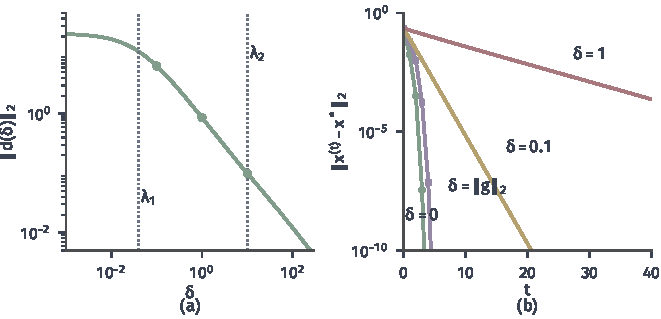
\includegraphics[width=112mm]{figures/05-optimization/02-smooth-optimization/matplotlib/newton-shift-effects/figure.pdf}
  \caption{对角平移的两个效应。(a)在$(-1,\tfrac65)$处方向长度随$\delta$的变化，灰色竖线是Hessian的两个特征值，绿点对应$\delta=0.1,1,10$。(b)从$(0.9,0.8)$出发、使用完整步的距离误差：绿线$\delta=0$，紫线$\delta=\lVert\bm{g}\rVert_2$，黄线$\delta=0.1$，红线$\delta=1$。修正量不消失时收敛只有线性。}
  \label{fig:newton-shift-effects}
\end{BookInlineFigure}

实际上不必先算$\lambda_{\min}$。尝试对$\bm{H}^{(t)}+\delta\bm{I}$作Cholesky分解：分解成功说明已经正定，遇到非正主元就增大$\delta$再试。这正是后面计算过程采用的做法。

\paragraph{谱修正}
对角平移把所有特征值一起抬高，也改动了本来很好的方向。如果能算出谱分解$\bm{H}^{(t)}=\bm{Q}\bm{\Lambda}\bm{Q}^\top$，就可以只改有问题的特征值，这称为\term{谱修正}（spectral modification）：
\begin{equation}
 \bm{B}^{(t)}=\bm{Q}\tilde{\bm{\Lambda}}\bm{Q}^\top,\qquad
 \tilde\lambda_i=\max\bigl\{\lvert\lambda_i\rvert,\ \epsilon\bigr\}.
 \label{eq:newton-spectral}
\end{equation}
其中$\epsilon>0$是下限。取绝对值的含义是：负曲率方向上，模型的碗是倒扣的，那就翻过来，弯度的大小不变。Newton方向在这个特征方向上的分量$-\bm{q}_i^\top\bm{g}/\lambda_i$指向鞍点，翻转后变为$-\bm{q}_i^\top\bm{g}/\lvert\lambda_i\rvert$，朝下坡方向走。

图~\ref{fig:newton-spectral-maps}比较三种常见的特征值映射。只把小于下限的值截到$\epsilon$也是一种选择，但在负曲率方向上会得到很大的步。在$(-\tfrac12,\tfrac34)$处，取$\epsilon=0.1$的截断规则给出的方向是$(7.87,-6.32)$，比取绝对值得到的$(1.33,-1.21)$长了好几倍。

\begin{BookInlineFigure}
  \centering
  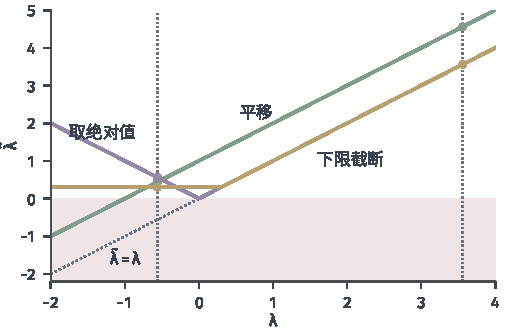
\includegraphics[width=86mm]{figures/05-optimization/02-smooth-optimization/matplotlib/newton-spectral-maps/figure.pdf}
  \caption{特征值$\lambda$经修正后的值$\tilde\lambda$。绿线是平移$\delta=1$，紫线是取绝对值，黄线是下限截断$\max\{\lambda,0.3\}$，灰色点线是不修正。竖线标出$(-\tfrac12,\tfrac34)$处Hessian的两个特征值，三条线上的点是修正后的值。红色浅底是不允许的非正区域。}
  \label{fig:newton-spectral-maps}
\end{BookInlineFigure}

谱修正的修正量最贴合问题，但要计算完整的特征分解，稠密时的常数比Cholesky分解大得多。

\paragraph{修正Cholesky分解}
第三种做法把修正放进分解过程。在作$\bm{L}\bm{D}\bm{L}^\top$分解时，第$j$步的主元$c_j$如果太小或为负，就把它换成正数，分解继续往下走。这称为\term{修正Cholesky分解}（modified Cholesky factorization），得到的$\bm{B}=\bm{L}\bm{D}\bm{L}^\top$自动正定，分解已经完成，成本与普通分解同量级。

在$(-\tfrac12,\tfrac34)$处。第一个主元是$c_1=1$，消元乘子是$\ell_{21}=2$，第二个主元是
\[
 c_2=2-\ell_{21}^2c_1=2-4=-2.
\]
这个主元为负，普通Cholesky分解在此失败。把它换成绝对值$d_2=2$，得到
\[
 \bm{B}=\begin{bmatrix}1&0\\2&1\end{bmatrix}
 \begin{bmatrix}1&0\\0&2\end{bmatrix}
 \begin{bmatrix}1&2\\0&1\end{bmatrix}
 =\begin{bmatrix}1&2\\2&6\end{bmatrix}.
\]
相当于只修改了右下角元素，$\bm{E}=\operatorname{diag}(0,4)$。

简单地“遇到负主元就取绝对值”可能带来很大的修正，因为小主元会放大后面的元素。取
\[
 \bm{H}=\begin{bmatrix}0.01&1\\1&0\end{bmatrix},
\]
它的特征值约为$\pm1$，平移量$1$多一点就够。可是$c_1=0.01$是正的，不作修改，于是$\ell_{21}=100$，$c_2=0-100^2\times0.01=-100$。取绝对值之后$\bm{B}$的右下角是$\ell_{21}^2c_1+d_2=200$，修正量高达$200$。

办法是同时限制消元乘子的大小。记$\theta_j=\max_{i>j}\lvert c_{ij}\rvert$为第$j$列主元下方尚未除以主元的元素的最大绝对值，给定上界$\bar\beta>0$和下限$\hat\delta>0$，取
\begin{equation}
 d_j=\max\Bigl\{\lvert c_j\rvert,\ \frac{\theta_j^2}{\bar\beta^2},\ \hat\delta\Bigr\}.
 \label{eq:newton-modified-cholesky-pivot}
\end{equation}
上面的例子取$\bar\beta=1$。第一列$\theta_1=1$，所以$d_1=\max\{0.01,1,\hat\delta\}=1$，$\ell_{21}=1$。第二个主元是$c_2=0-1=-1$，$d_2=1$。最后得到
\[
 \bm{B}=\begin{bmatrix}1&1\\1&2\end{bmatrix},\qquad \bm{E}=\operatorname{diag}(0.99,\,2).
\]
修正量降到与$\lvert\lambda_{\min}\rvert$同一量级。参数怎样选择才能在理论上控制$\lVert\bm{E}\rVert$，证明较长，读者可查阅\scite{math-nocedal2006numerical}。

\paragraph{三种修正的比较}
图~\ref{fig:newton-directions}和表~\ref{tab:newton-correction-compare}在同一点比较三种修正。三个方向都转向了下坡，都需要回溯一次，$\alpha=1$都被拒绝，$\alpha=\tfrac12$都被接受。这一点上修正Cholesky分解的新点目标值最低，这只是这一步的结果，不代表它总是更好。

\begin{BookInlineFigure}
  \centering
  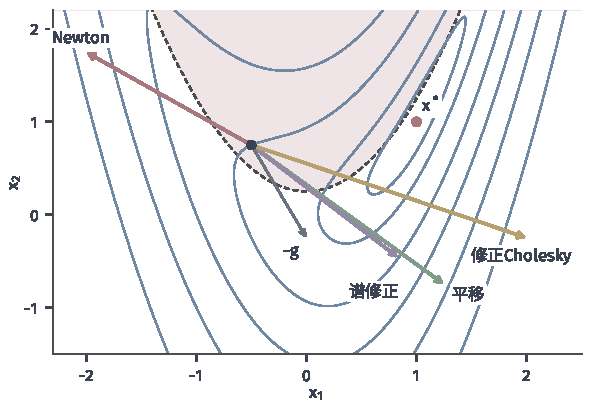
\includegraphics[width=100mm]{figures/05-optimization/02-smooth-optimization/matplotlib/newton-directions/figure.pdf}
  \caption{$\bm{x}=(-\tfrac12,\tfrac34)$（黑点）处的几种方向，箭头按实际长度绘制。红色是未修正的Newton方向，指向上坡。绿色、紫色、黄色分别是对角平移$\delta=1$、谱修正（取绝对值）、修正Cholesky分解得到的方向，灰色是负梯度。蓝线是等高线，红色浅底是Hessian不定的区域，红点是解。}
  \label{fig:newton-directions}
\end{BookInlineFigure}

\begin{BookInlineTable}
  \centering
  \begin{tabular}{@{}lccccc@{}}
    \toprule
    做法 & $\lVert\bm{E}\rVert_2$ & $\bm{d}$ & $\bm{g}^\top\bm{d}$ & $\alpha$ & 新点$f$ \\
    \midrule
    对角平移$\delta=1$ & $1$ & $(1.75,-1.5)$ & $-2.375$ & $\tfrac12$ & $0.2151$ \\
    谱修正（绝对值） & $1.123$ & $(1.334,-1.213)$ & $-1.880$ & $\tfrac12$ & $0.3604$ \\
    修正Cholesky & $4$ & $(2.5,-1)$ & $-2.25$ & $\tfrac12$ & $0.1289$ \\
    \bottomrule
  \end{tabular}
  \caption{在$(-\tfrac12,\tfrac34)$处三种修正的结果，出发点目标值$1.375$，回溯参数$c=0.1$，$\beta=0.5$。}
  \label{tab:newton-correction-compare}
\end{BookInlineTable}

\paragraph{计算过程}
下面以对角平移为例写出完整算法，它只用Cholesky分解试探，不需要特征值。$\delta$的试探规则如下：对角元都为正时从$0$开始试；否则从$-\min_ih_{ii}+b$开始，$b>0$是一个固定的基准量；分解失败时令$\delta\leftarrow\max\{2\delta,b\}$。

\needspace{6\baselineskip}
\paragraph{变量}
\begin{itemize}
 \item $\bm{x},\bm{g},\bm{H}$：当前点、梯度、Hessian。
 \item $\delta$：本轮的对角平移量，每轮重新确定。
 \item $\bm{L}$：$\bm{H}+\delta\bm{I}$的Cholesky因子。
 \item $\bm{d}$：修正后的方向。
 \item $\alpha,c,\beta$：回溯所用的量，与上一节相同。
 \item $b$：平移基准量，例中取$1$。
\end{itemize}

\paragraph{初始化}
选定$\bm{x}^{(0)}$和各参数。例中取下面的数据：
\[
 \bm{x}^{(0)}=\bigl(-\tfrac12,\tfrac34\bigr),\qquad b=1,\qquad c=0.1,\qquad \beta=0.5,\qquad \varepsilon=10^{-6}.
\]

\needspace{6\baselineskip}
\paragraph{每轮更新}
在第$t$轮：
\begin{enumerate}
 \item \textbf{读取导数并检查停止。}计算$\bm{g}^{(t)}$、$\bm{H}^{(t)}$，若$\lVert\bm{g}^{(t)}\rVert_2\leq\varepsilon$，输出$\bm{x}^{(t)}$并结束。

 例中第一轮的数据已在本节开头列出。

 \item \textbf{确定平移量。}按上述规则试探，直到Cholesky分解成功，得到$\delta^{(t)}$和$\bm{L}$。

 例中第一轮对角元都为正，先试$\delta=0$，第二个主元$2-4=-2$，分解失败。再试$\delta=1$，矩阵和因子为
 \[
  \bm{H}+\bm{I}=\begin{bmatrix}2&2\\2&3\end{bmatrix},\qquad
  \bm{L}=\begin{bmatrix}\sqrt2&0\\\sqrt2&1\end{bmatrix},
 \]
 分解成功，$\delta^{(0)}=1$。

 \item \textbf{求方向。}前代、回代解方程~\eqref{eq:newton-modified-equation}。

 例中第一轮解$2d_1+2d_2=\tfrac12$，$2d_1+3d_2=-1$，得到
 \[
  \bm{d}^{(0)}=\begin{bmatrix}1.75\\-1.5\end{bmatrix}.
 \]

 \item \textbf{回溯并更新。}从$\alpha=1$开始按式~\eqref{eq:newton-armijo}回溯，然后更新$\bm{x}$，令$t\leftarrow t+1$。

 例中第一轮方向导数为$-2.375$。试$\alpha=1$，新点目标值$5.379$，高于右端$1.1375$，拒绝。试$\alpha=\tfrac12$，新点是$(\tfrac38,0)$，目标值$0.2151$，低于右端$1.2563$，接受。

 第二轮$u=-\tfrac9{64}$，$1-4u=\tfrac{25}{16}>0$，Hessian已经正定，$\delta^{(1)}=0$的分解成功。方向就是Newton方向，由式~\eqref{eq:newton-running-direction}，
 \[
  d_1=\frac{5/8}{25/16}=\frac25,\qquad d_2=\frac9{64}+\frac34\cdot\frac25=0.440625.
 \]
 完整步被接受，到达$(0.775,0.440625)$，目标值$0.0509$。
\end{enumerate}

各轮结果见表~\ref{tab:newton-modified-run}。修正只在第一轮出现，第$6$轮梯度范数低于容差，迭代结束，最终得到$\bm{x}^{(6)}\approx(1,1)$。图~\ref{fig:newton-modified-path}是这条路径。

\begin{BookInlineTable}
  \centering
  \begin{tabular}{@{}ccccc@{}}
    \toprule
    $t$ & $\bm{x}^{(t)}$ & $f$ & $\delta^{(t)}$ & $\alpha^{(t)}$ \\
    \midrule
    $0$ & $(-0.5,0.75)$ & $1.375$ & $1$ & $1/2$ \\
    $1$ & $(0.375,0)$ & $0.2151$ & $0$ & $1$ \\
    $2$ & $(0.775,0.4406)$ & $0.05091$ & $0$ & $1$ \\
    $3$ & $(0.9122,0.8133)$ & $4.21\mathrm{e}{-3}$ & $0$ & $1$ \\
    $4$ & $(0.9939,0.9811)$ & $6.34\mathrm{e}{-5}$ & $0$ & $1$ \\
    $5$ & $(0.99984,0.99965)$ & $1.40\mathrm{e}{-8}$ & $0$ & $1$ \\
    $6$ & $(1.0000,1.0000)$ & $9.1\mathrm{e}{-16}$ & 停止 & \\
    \bottomrule
  \end{tabular}
  \caption{对角平移的修正Newton法从$(-\tfrac12,\tfrac34)$出发的迭代，只有第一轮需要修正和回溯。}
  \label{tab:newton-modified-run}
\end{BookInlineTable}

\begin{BookInlineFigure}
  \centering
  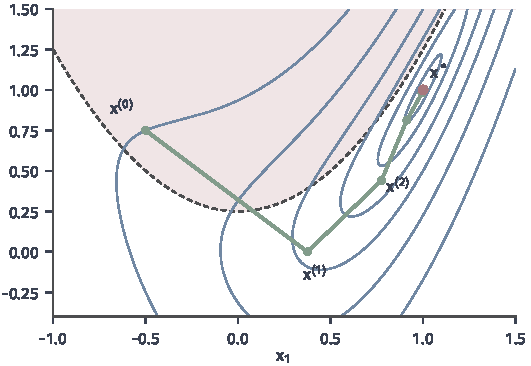
\includegraphics[width=90mm]{figures/05-optimization/02-smooth-optimization/matplotlib/newton-modified-path/figure.pdf}
  \caption{修正Newton法的路径（绿）。起点$(-\tfrac12,\tfrac34)$在Hessian不定的红色浅底区域内，第一步用$\delta=1$的修正方向并取步长$\tfrac12$，落入正定区域后修正消失，以后都是完整的Newton步。蓝线是等高线，红点是解。}
  \label{fig:newton-modified-path}
\end{BookInlineFigure}

\paragraph{全局性质：一致有界的修正}
修正之后方向不再是Newton方向，上一节的定理不能直接用。下面的结论只要求修正后的矩阵特征值一致有界，不要求目标凸，这正是修正要达到的目的。

\begin{theorem}[修正方向的全局收敛]
\label{thm:newton-modified-global}
设$f$有下界，$\nabla f$是$L$-Lipschitz的，存在$0<b\leq\bar b$，使各轮$b\bm{I}\preceq\bm{B}^{(t)}\preceq\bar b\bm{I}$。方向由方程~\eqref{eq:newton-modified-equation}给出，步长由Armijo回溯确定，$c\in(0,1)$，$\beta\in(0,1)$，初始试探为$1$。记
\begin{equation}
 \alpha_{\min}=\min\Bigl\{1,\ \frac{2\beta(1-c)b^2}{L\bar b}\Bigr\}.
 \label{eq:newton-alpha-min}
\end{equation}
则
\begin{equation}
 \min_{0\leq t\leq T}\lVert\bm{g}^{(t)}\rVert_2^2\leq\frac{\bar b\,\bigl(f(\bm{x}^{(0)})-\inf f\bigr)}{c\,\alpha_{\min}\,(T+1)}.
 \label{eq:newton-modified-rate}
\end{equation}
特别地，$\lVert\bm{g}^{(t)}\rVert_2\to0$。
\end{theorem}

\begin{proof}
省略上标。梯度$L$-Lipschitz给出二次上界
\[
 f(\bm{x}+\alpha\bm{d})\leq f(\bm{x})+\alpha\bm{g}^\top\bm{d}+\frac L2\alpha^2\lVert\bm{d}\rVert_2^2.
\]
与Armijo条件比较，只要
\[
 \alpha\leq\frac{2(1-c)\lvert\bm{g}^\top\bm{d}\rvert}{L\lVert\bm{d}\rVert_2^2},
\]
条件就成立。

由特征值的界，方向导数和方向长度满足
\[
 \lvert\bm{g}^\top\bm{d}\rvert=\bm{g}^\top\bm{B}^{-1}\bm{g}\geq\frac{\lVert\bm{g}\rVert_2^2}{\bar b},\qquad
 \lVert\bm{d}\rVert_2\leq\frac{\lVert\bm{g}\rVert_2}{b}.
\]
于是上述门槛不小于$2(1-c)b^2/(L\bar b)$。回溯的步长要么是初始的$1$，要么是一个被拒绝的值乘以$\beta$，所以$\alpha\geq\alpha_{\min}$。

代入Armijo条件，每轮下降量满足
\[
 f(\bm{x})-f(\bm{x}^{(t+1)})\geq c\,\alpha_{\min}\frac{\lVert\bm{g}\rVert_2^2}{\bar b}.
\]
对$t=0,\ldots,T$求和，左端不超过$f(\bm{x}^{(0)})-\inf f$，最小值不超过平均值，即得式~\eqref{eq:newton-modified-rate}。由于级数$\sum_t\lVert\bm{g}^{(t)}\rVert_2^2$收敛，通项趋于零。
\end{proof}

结论只说梯度趋于零，极限点可能是鞍点。在鞍点处$\bm{g}^{(t)}=\bm{0}$，方程~\eqref{eq:newton-modified-equation}的解是零向量，无论怎样修正都不会动。怎样从鞍点离开，是第~\ref{chap:saddle-points}章的问题。

\paragraph{修正何时消失}
修正对局部速度的影响可以精确写出来。设$\bm{e}=\bm{x}^{(t)}-\bm{x}^\star$，$\bm{B}=\bm{H}^{(t)}+\bm{E}$，步长为$1$。照定理~\ref{thm:newton-local}证明的做法，得到
\[
 \bm{x}^{(t+1)}-\bm{x}^\star=\bm{B}^{-1}\Bigl[\int_0^1\bigl(\bm{H}^{(t)}-\nabla^2f(\bm{x}^\star+s\bm{e})\bigr)\bm{e}\,\mathrm{d}s+\bm{E}\bm{e}\Bigr].
\]
方括号中第一项是模型的二次误差，第二项是修正带来的一次误差。若$\lVert\bm{B}^{-1}\rVert_2$一致有界，就得到
\begin{equation}
 \lVert\bm{x}^{(t+1)}-\bm{x}^\star\rVert_2\leq\lVert\bm{B}^{-1}\rVert_2\Bigl(\frac M2\lVert\bm{e}\rVert_2^2+\lVert\bm{E}\rVert_2\lVert\bm{e}\rVert_2\Bigr).
 \label{eq:newton-modified-local}
\end{equation}

由此可以逐条读出修正的三种结局。若$\bm{E}$有限步后为零，则恢复二次收敛。若修正量趋于零，收敛是超线性的。若修正量与误差同阶，仍然是二次收敛。修正量不消失时只有线性收敛：在特征值为$\lambda$的方向上，$\bm{E}=\delta\bm{I}$的误差因子是$\delta/(\lambda+\delta)$。

主例解处的小特征值约为$0.185$。取$\delta=0.1$时因子约$0.35$，取$\delta=1$时约$0.84$，图~\ref{fig:newton-shift-effects}(b)中黄线和红线的斜率正是如此。紫线取$\delta=\lVert\bm{g}\rVert_2$，修正量随误差同阶消失，仍然以二次速度收敛。

所以修正Newton法必须满足一个要求：Hessian足够正定时要退回不修正。上面的试探规则总是先试$\delta=0$，正好满足这一点。若$\nabla^2f(\bm{x}^\star)\succ\bm{0}$，在解附近分解一次成功，迭代就成为纯粹的Newton法。使用谱修正时，下限$\epsilon$要小于$\lambda_{\min}(\nabla^2f(\bm{x}^\star))$，否则修正不会消失。

\paragraph{改迭代与改目标}
把$\bm{H}^{(t)}$换成$\bm{H}^{(t)}+\delta\bm{I}$，方程很像给目标加了正则项$\tfrac\delta2\lVert\bm{x}\rVert_2^2$之后的Newton方程，两件事却完全不同。下面用一元目标$f(x)=\tfrac12(x-1)^2$比较。

修正迭代时，$x^{(t+1)}=x^{(t)}-(x^{(t)}-1)/(1+\delta)$，极限仍是$1$，只是收敛变慢。改目标时，新目标的最小点是$1/(1+\delta)$，解已经变了。

\begin{BookInlineTable}
  \centering
  \begin{tabular}{@{}lll@{}}
    \toprule
    & 修正迭代 & 改变目标 \\
    \midrule
    方程右端 & 原梯度$-\bm{g}^{(t)}$ & 新目标的梯度$-\bm{g}^{(t)}-\delta\bm{x}^{(t)}$ \\
    驻点 & 与原目标相同 & 通常移动 \\
    作用 & 让方向可用 & 改变要解的问题 \\
    \bottomrule
  \end{tabular}
  \caption{曲率修正和正则化的区别。修正只影响路径，不影响梯度为零的点。}
  \label{tab:newton-modify-vs-regularize}
\end{BookInlineTable}

平移量$\delta$还可以根据模型预测准不准来自动调整，这与直接限制位移的长度密切相关，将在第~\ref{chap:trust-region}章讨论。
